\documentclass{article}

\usepackage[most]{tcolorbox}
\usepackage{physics}
\usepackage{graphicx}
\usepackage{float}
\usepackage{amsmath}
\usepackage{amssymb}


\usepackage[utf8]{inputenc}
\usepackage[a4paper, margin=1in]{geometry} % Controla los márgenes
\usepackage{titling}

\title{Clase 8 }
\author{Manuel Garcia.}
\date{\today}

\renewcommand{\maketitlehooka}{%
  \centering
  \vspace*{0.05cm} % Espacio vertical antes del título
}

\renewcommand{\maketitlehookd}{%
  \vspace*{2cm} % Espacio vertical después de la fecha
}

\newcommand{\caja}[3]{%
  \begin{tcolorbox}[colback=#1!5!white,colframe=#1!25!black,title=#2]
    #3
  \end{tcolorbox}%
}

\begin{document}
\maketitle

\section{Ejemplo 1}
Para oscilador armonico clásico de $ m  $ grados de libertas, determine el volumen en el espacio de fase y su trayectoria clásica.

\begin{gather*}
  H(p,q) = \frac{p^2 }{2m } + \frac{1}{2} m \omega ^2 q ^2 ; \qquad \qquad \omega ^2 = \frac{k}{m } 
\end{gather*}

 Para unas condiciones iniciales dadas por $ t_0; \qquad q = A; \qquad p = 0  $ 

 \hfill 

 \hfill 

\textbf{Solucion }

 Dado que $ H(p, q) = \epsilon $; energia mecánica total 
 \begin{gather*}
   \frac{p^2 }{2m } + \frac{1}{2} m \omega ^2 q ^2 = \epsilon \rightarrow \frac{p^2 }{2m\epsilon } + \frac{q ^2 }{\frac{2\epsilon }{m \omega ^2}} = 1\\
   \rightarrow \frac{p _{\omega} ^2}{b ^2} + \frac{q_\omega ^2}{a ^2} = 1
 \end{gather*}

 Trayectoria en el espacio de fase: 
 \begin{figure}[H]
  \begin{center}
    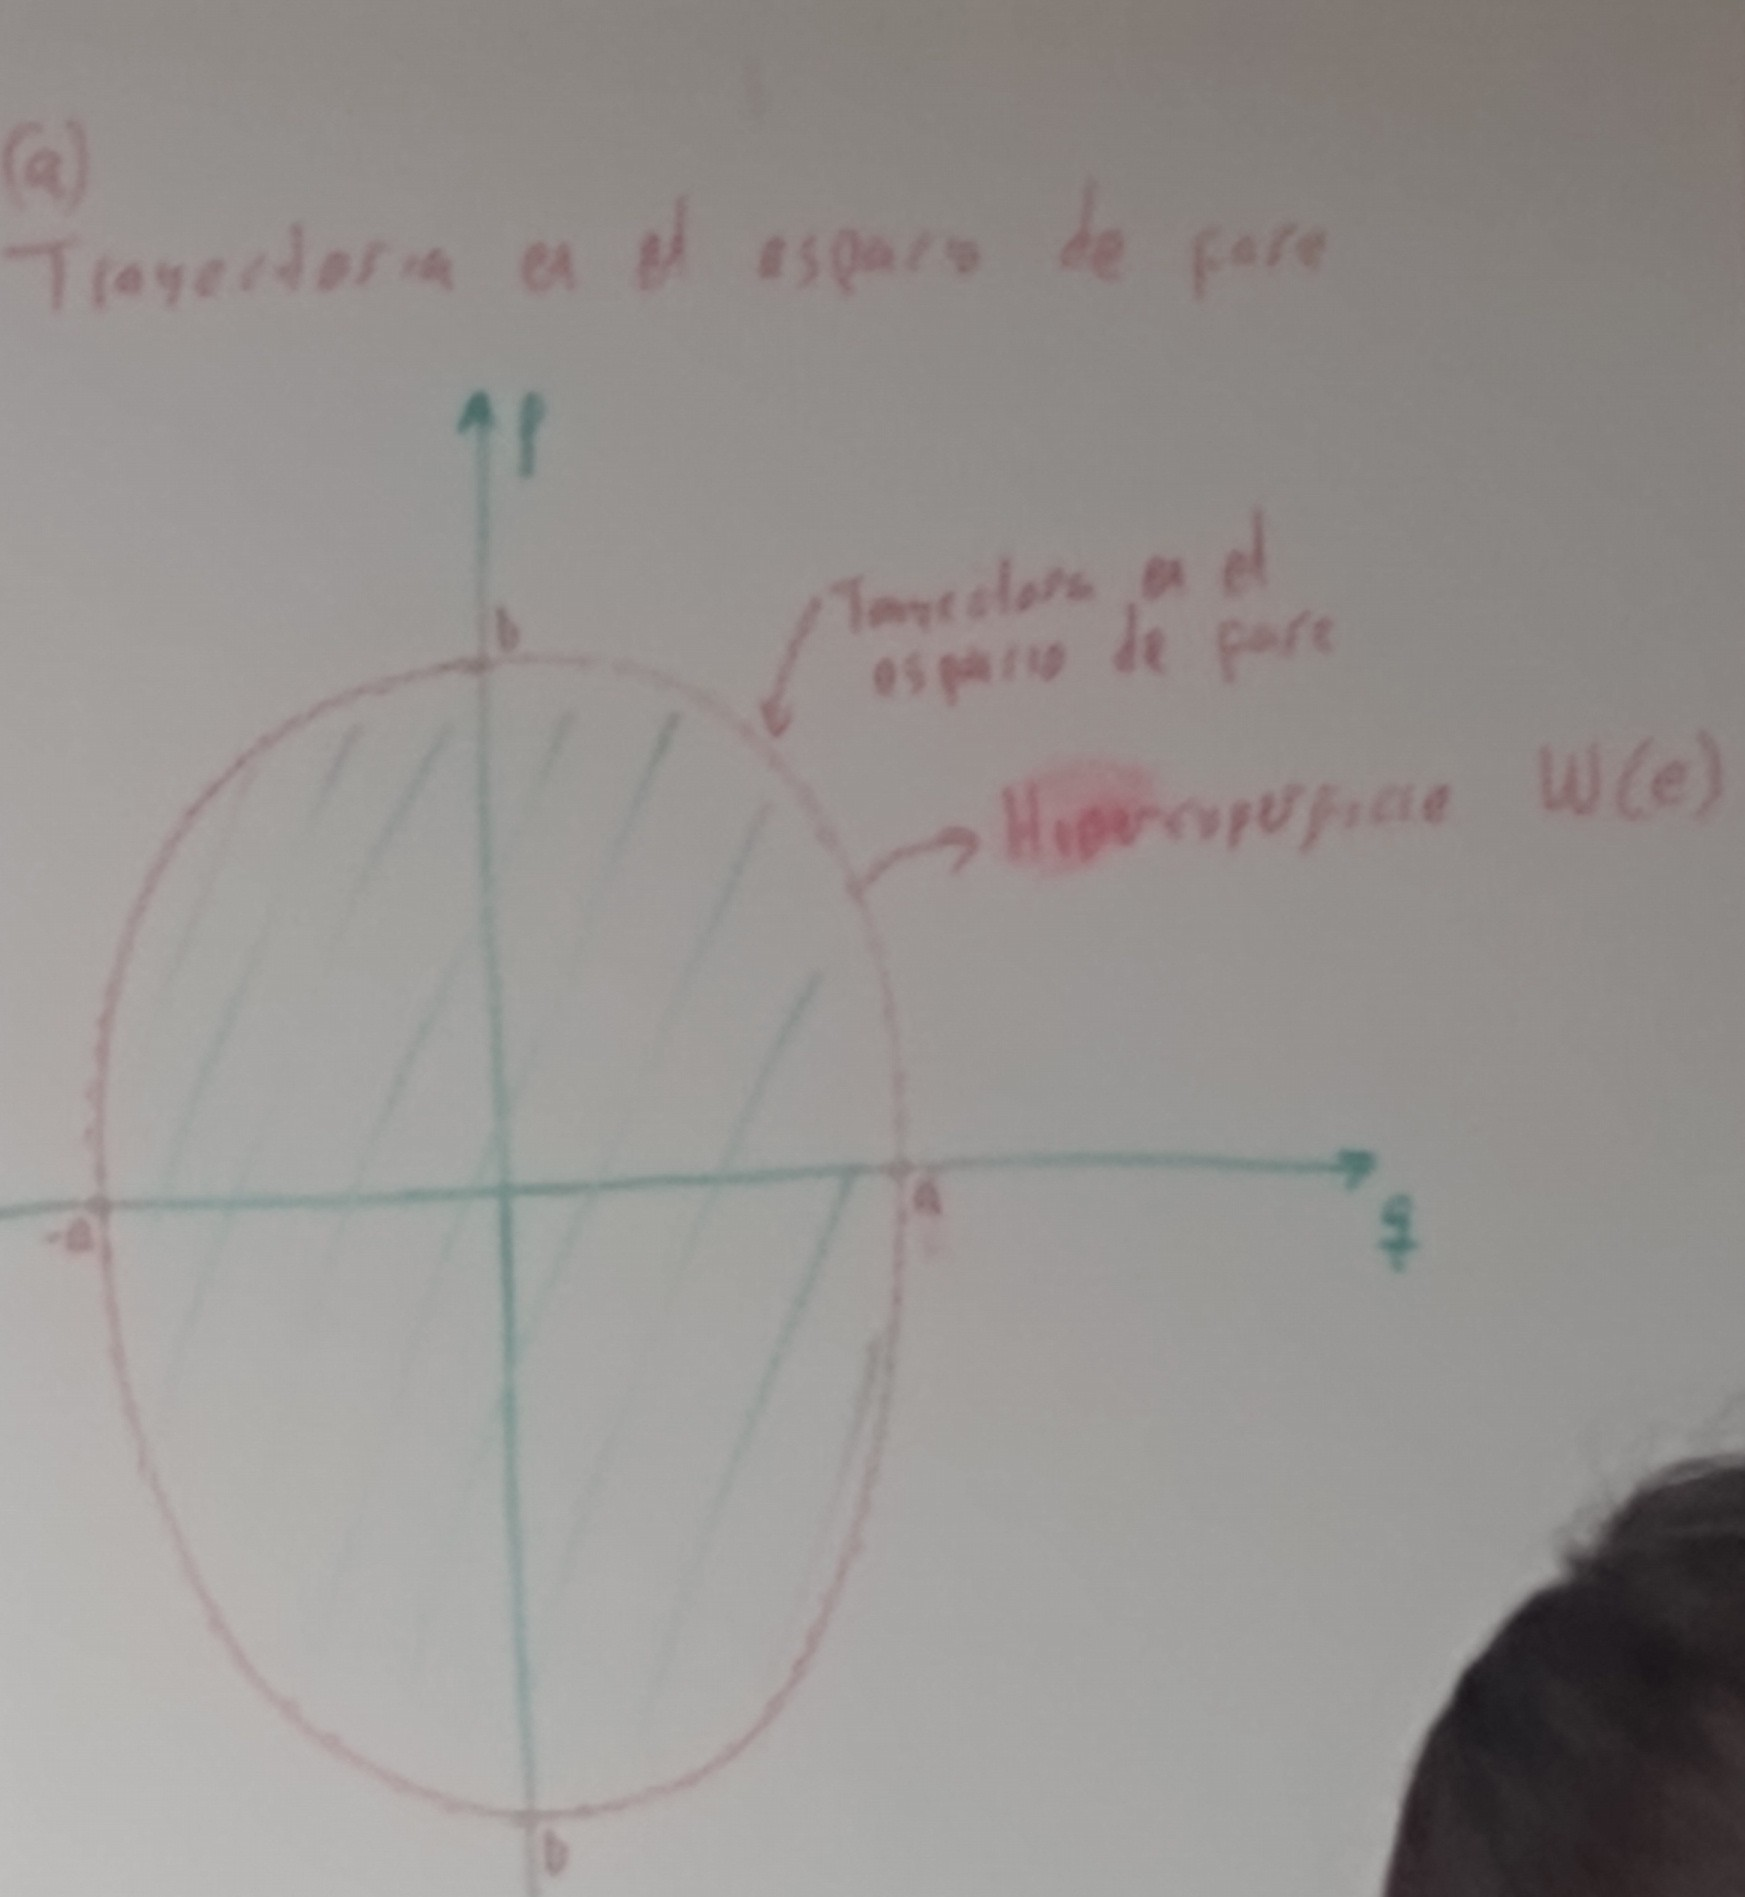
\includegraphics[width=0.4\textwidth]{espacio_fase.jpg}
  \end{center}
\end{figure}



El volumen $ \Lambda(\epsilon) $ está envuelto por la hipersuperficie $ \omega(\epsilon) $. El area de esta es el area de la elipse. 
\begin{gather*}
  \Lambda(\epsilon) = \pi ab = \pi \sqrt{\frac{2\epsilon}{m \omega^2 }}  \sqrt{2m\epsilon} \\
  \Lambda(\epsilon) = 2\pi \frac{\epsilon}{\omega}
\end{gather*}

De forma equivalente 
\begin{gather*}
  p ^2 = 2m\epsilon - \frac{1}{2} m^2 \omega ^2 q ^2 \quad \rightarrow \quad \left|p \right| = \sqrt{2m\epsilon - \frac{1}{2} m^2 \omega ^2 q ^2} \\
  \Lambda(\epsilon) = \int_{H(p,q)\leq \epsilon}^{} d\Lambda = \int_{-A }^{A }dq \int_{- \left|p \right|}^{\left|p \right|} = 4 \int_{0 }^{A } dq \int_{0 }^{\left|p \right|}dp \\
  \Lambda(\epsilon) = 4 \int_{0 }^{A } dq \sqrt{2m\epsilon - \frac{1}{2} m \omega ^2 q ^2} = 4 \sqrt{2m \epsilon} \int_{0 }^{A } dq \sqrt{1- D q ^2} \qquad \text{con }D = \frac{1}{2} \frac{m \omega ^2}{\epsilon}\\
  = \sqrt{2m \epsilon} \frac{1}{2} \left[ A \sqrt{1 - A ^2 D } + \frac{\arcsin{A \sqrt{D } }}{\sqrt{D } }\right]  \\
  \text{Tenemos que } \frac{\arcsin A \sqrt{D } }{\sqrt{D } } = \frac{\pi}{2} \sqrt{\frac{2 \epsilon}{m\omega} } , \qquad A = \frac{2\epsilon}{m \omega^2}\\
  \Lambda(\epsilon) = 2\pi \frac{\epsilon}{\omega}
\end{gather*}

\hfill 

\hfill 

si $ \epsilon \rightarrow \epsilon' = \epsilon + \Delta \epsilon $ 
\begin{gather*}
  \Lambda = 2\pi \frac{\epsilon' }{\omega} = 2\pi \frac{\epsilon}{\omega} + 2\pi \frac{\Delta \epsilon}{\omega}\\
  \Delta \Lambda = \Lambda' - \Lambda \\
  \Delta \Lambda  = 2\pi \frac{\Delta \epsilon}{\omega}
\end{gather*}

\section{Ejemplo 2 }
Asumamos que la probabilidad de encontrar al oscilador con un $ q  $ entre $ q  $ y $ q+dq  $ está dada por 
\begin{gather*}
  \rho(q) dq = \frac{d \Lambda}{\Delta \Lambda}
\end{gather*}
Encuentre $ \rho(q )  $ como funcion de $ A  $ (amplitud)

Así: 
\begin{gather*}
  \rho(q) dq = \frac{2 dp dq }{2\pi \frac{\Delta\epsilon}{\omega}} = \frac{\omega}{\pi} dp \frac{dq }{d\epsilon} = \frac{\omega}{\pi} \left(\frac{dp }{d\epsilon}\right)dq  
\end{gather*}

y que $ \epsilon = \epsilon (p,q) = \frac{p ^2}{2m } + \frac{1}{2} m \omega^2 q^2  $ 

$ \frac{d \epsilon }{d p } = \frac{1}{2m }2 \left|p \right| = \frac{\left|p \right|}{m } \rightarrow \frac{d p  }{d \epsilon} = \frac{m }{\left|p \right|} $

\hfill 

Así $  \rho(q) = \frac{\omega}{\pi} \frac{d p  }{d \epsilon} = \frac{\omega}{\pi} \frac{m }{\left|p \right|} =\frac{\omega}{\pi} \frac{m }{\sqrt{2m\epsilon - \frac{1}{2} m^2 \omega ^2 q ^2}} $

\hfill 

\hfill 

tenemos que 
\begin{gather*}
  q^2 = A^2 \cos^2{(\omega t + \phi)}
  \dot q^2 = A^2 \sin^2{(\omega t + \phi)}
\end{gather*}
Luego 
\begin{gather*}
  \tilde p = m ^2 \dot q^2 = A^2 m^2 \omega^2   \sin^2{(\omega t + \phi)}
\end{gather*}
Así 
\begin{gather*}
  \epsilon = \frac{1}{2m } p^2 + \frac{1}{2} m \omega^2 q^2 = \frac{1}{2} A^2 m \omega^2 \quad \rightarrow \quad A^2 = \frac{2 \epsilon}{m \omega^2 } 
\end{gather*}
Entonces 
\begin{gather*}
  m^2 \omega^2 A^2 = 2m \epsilon 
\end{gather*}

\caja{green}{Ejercicio }{
Si $ q(t) = A \cos{(\omega t + \phi )} $, $ 0 <\phi<2\pi $ asumiendo que $ \omega(\phi )d\phi  $ es la probabilidad de que $ \phi  $ se encuentre entre $ \phi  $ y $ \phi + d\phi  $ es: 
\begin{gather*}
  \omega(\phi) d\phi = \frac{1}{2\pi } d \phi  
\end{gather*}
Establecida la correspondencia con la probabilidad de que $ q  $ se encuentre entre $ q  $ y $ q + d q  $ dad por $ p (q) dq  $, encontrar 
\begin{gather*}
  \rho(q) 
\end{gather*}
}


\section{Ejemplo 3 } 

\hfill

\textbf{(a)} Encontrar el volumen en el espacio de fase para un pendulo simple con pequeñas oscilaciones de longitud $ l  $ y masa $ m  $

\textbf{(b)} Determine el cambio en el volumen en el espacio de fase $ \Delta \Lambda $ si la longitud del pendulo cambia de $ l \rightarrow l' = 2l  $

\textbf{Solucion }
La energia 
\begin{gather*}
  E = T+V = \frac{1}{2} m v^2 + m gl (1- \cos{\theta}) = \frac{ml^2 \dot \theta^2 }{2} + m \omega^2 l^2 (1 - \cos{\theta }); \qquad \omega^2 = \frac{g}{l } 
\end{gather*}
\textbf{(a)} Para pequeñas oscilaciones $ \cos{\theta} \approx 1 - \frac{\theta^2 }{2! } + \cdots  $
\begin{gather*}
  \frac{1}{2} m A^2 \omega^2 = \frac{p_\theta^2 }{2m l^2 } + \frac{m \omega^2 l^2 \theta^2 }{2 } \\
  \rightarrow \quad 1 = \frac{p_\theta^2 }{(ml\omega A)^2 } + \frac{\theta^2 }{(A/l)^2 } = \frac{p_\theta^2 }{b^2 } + \frac{\theta^2 }{a^2 }
\end{gather*}
Volumen $ \Lambda $ envuelto por $ \omega(\epsilon) $ 
\begin{gather*}
  \Lambda = \pi ab = \pi m \omega A^2  
\end{gather*}

\section{Ejemplo 4 }
Considerando el oscilador armónico cuántico, determine el minimo elemento de volumen en el espacio de fase por un estado cuantico arbitrario (i-esimo) $ \rightarrow \ket{\phi_i } \rightarrow \epsilon_i = \hbar  \omega (i + 1/2 ) $.

El hamiltoniano del sistema 
\begin{gather*}
  H ^ {(1) } = \frac{\hat p ^2 }{2m } + \frac{1}{2} m \omega^2 \hat x ^2 ; \qquad \qquad \omega^2 = \frac{k }{m } 
\end{gather*}

\textbf{Solucion } 
\begin{gather*}
  \hat H ^ {(1) } \ket{\phi_i }= \epsilon_i \ket{\phi_i }; \qquad  \epsilon_i = \hbar  \omega (i + 1/2 )
\end{gather*}
Dado que el hamiltoniano representa la energia mecanica total 
\begin{gather*}
  \epsilon_i = \frac{p^2 }{2m } + \frac{1}{2} m \omega^2 q^2  
\end{gather*}
El volumen en el espacio de fase 
\begin{gather*}
  \Lambda_i = \int_{H(p,q) \leq \epsilon_i }^{}d\Lambda_i = \int_{}^{} dq \int_{H(p,q) \leq \epsilon_i }^{} dp  
\end{gather*}
Los limites de la integral 
\begin{gather*}
  \epsilon_i = \frac{1}{2} m \omega^2 q^2 ; \qquad \text{para }q = 0 \\
  q^2 = \frac{2 \epsilon_i }{m \omega^2 } \quad \rightarrow \quad q = \pm \sqrt{\frac{2 \epsilon_i }{m \omega^2 }} = \pm A_i 
\end{gather*}

\hfill 

\hfill 

\hfill 

\begin{gather*}
  p^2 = 2m \epsilon_i - m \omega^2 q^2 \quad \rightarrow \quad p = \pm \sqrt{2m \epsilon_i - m^2 \omega^2 q^2 } = \pm \left|p \right| 
\end{gather*}

Entonces 
\begin{gather*}
  \Lambda_i = 4 \int_{0 }^{A } dq \int_{0 }^{\left|p \right|} dp = \frac{2\pi}{\omega} \epsilon_i \\
  \Lambda_i = \frac{2\pi}{\omega} \hbar \omega(i + \frac{1}{2}) = h (i + \frac{1}{2})
\end{gather*}
Para el estado base $ i = 0  $ 
\begin{gather*}
  \Lambda_0 = \frac{h }{2} \quad \rightarrow \quad \frac{\Lambda_0 }{2 } = h  
\end{gather*}
Por lo tanto 
\begin{gather*}
  \frac{\Lambda_i }{\left(i + \frac{1}{2}\right)} = h 
\end{gather*}


\section{Teorema de Virial }
Gas ideal de particulas libres 
\begin{gather*}
  H(p,q) = T(p) = \displaystyle\sum_{ l = 1 }^{ N } \frac{1}{2}m V_l^2 
\end{gather*}
Se calcula el promedio estadistico $ q_i \frac{\partial H  }{\partial q_k } $ en el ensamble microcaconico 

\begin{gather*}
  \rho(\vec q, \vec p ) = \frac{\delta (E- H)}{\omega(E)} 
\end{gather*}

Se calcula 
\begin{gather*}
  \bra{q_l }\ket{\frac{\partial H  }{\partial q_k }} = \int_{E- \Delta E < H < E + \Delta E }^{}  \frac{\delta (E- H)}{\omega(E)} q_l \frac{\partial H  }{\partial q_k } d \vec p d \vec q  = \delta _{lk } \frac{1}{\Omega h ^ {3\omega}} \int_{}^{}\cdots 
\end{gather*}

\begin{gather*}
  \bra{x_l }\ket{\frac{\partial H  }{\partial x_k }} = \delta _{lk }  \frac{1}{\Omega }\frac{\Lambda}{h ^ {3\omega}} = \delta _{lk } \frac{1}{\frac{\partial ln \Lambda }{\partial E }} = \delta _{lk } \frac{\kappa_B }{\left(\frac{\partial S  }{\partial E }\right) _{p,v} } = \delta _{lk } \delta_B   T
\end{gather*}

\begin{gather*}
  \bra{p_l }\ket{\frac{\partial H  }{\partial p_k }} = \delta _{lk }  \kappa_B T  
\end{gather*}

Usando el teorema de Euler 
\begin{gather*}
  2 T_x = \displaystyle\sum_{l }^{ } p_l \dot x_l \qquad \rightarrow \qquad \epsilon = \frac{1}{2} \kappa_b T  
\end{gather*}
Entonces 
\begin{gather*}
  \epsilon = \epsilon_x + \epsilon_y + \epsilon_z = \frac{3}{2}\kappa_B T 
\end{gather*}

\section{Ejemplo 6 }
Sea una cadena unidimensional que consiste de $ n \quad (n >> 1) $ elementos.


\end{document}
